% !TeX root = ../../../book.tex
\subsection{多项式}

有时我们需要使用平方、立方或更高次幂的变量。一般来说,多项式是我们用于表示一个函数的术语,该函数具有一个或多个整数次幂的变量,乘以系数,然后相加。以下是多项式的一些例子:
\[x^2 - 7x + 1,\quad 7p^6 + 5p^4 + 3p^2 + 2p,\quad \frac{1}{2}z^2 + 9y^2z - 2y + z^3y^2 - 7z\]

这些类型的函数在数学中非常常见和流行,部分原因是它们具有方便的属性,另一部分原因是它们在自然界中的普遍存在。我们将在本书中频繁地看到它们。不过,现在让我们将目光聚焦在只有一个\emph{输入变量}的多项式。

\subsubsection*{多项式的根}

有时,我们会在谜题中定义一个多项式函数,并想知道输入变量是否有任何值可以使输出值为 0。这些让输出值为 0 的输入值称为多项式的\textbf{根}。

识别多项式根的一种方法是将其隐式\textbf{因式分解}为线性项;也就是说,我们尝试将函数表示为一系列乘法而不是加法,因为我们可以声明(至少)其中一个因子为 $0$ 输出值才 $0$。该技术背后的动机依赖于以下事实:

\begin{quote}
    \textbf{事实:}如果 $a$ 和 $b$ 为实数且 $ab=0$,则 $a=0$ 或 $b=0$(或者两者都等于零)。
\end{quote}

\begin{example}
    我们来看一个具体的例子。尝试分解以下多项式:
    \[p(x) = x^2 + 6x + 8\]
    (将多项式定义为 $p(x)$ 是常见的表示法,其中 $p$ 代表多项式,$x$ 是输入变量,$p(x)$ 是与输入值 $x$ 对应的输出值。)

    你可能已经注意到
    \[p(x) = x^2 + 6x + 8 = (x + 4) \cdot (x + 2) = (x + 4)(x + 2)\]
    (当存在用括号分隔的因子时,删除 $\cdot$ 也是相当常见的,因此我们从现在开始也将采用该约定。)

    这种因式分解之所以有效,是因为我们多次相反地应用分配律。如果我们展开刚刚的因式分解,明确显示其中每一步,它看起来像:

    \begin{align*}
        p(x) &= (x + 4)(x + 2) \\
        &= x(x + 2) + 4(x + 2) \\
        &= (x^2 + 2x) + (4x + 8) \\
        &= x^2 + 2x + 4x + 8 = x^2 + 6x + 8
    \end{align*}

    我们真正写下因式分解步骤是为了注意到项 $+4$ 和 $+2$ 具有乘积 $+8$,这正是常数项,并且它们之和为 $+6$,而这正是 $x$ 项的系数。知道这些因式的后续展开如何进行,我们就可以在不进行检验的情况下写下因式分解。
\end{example}

\subsubsection*{二次因式分解}

让我们以上面示例为例,尝试推广到任何二次函数。如果我们想分解一个二次多项式
\[p(x) = x^2 + bx + c\]
我们要求 $r$ 和 $s$ 的值,使得 $r \cdot s = c$ 且 $r + s = b$。通常,我们可以``通过试算''来做到这一点,或者只需盯着这两个方程思考一分钟即可得出适当的值。(这就是我们在前一个例子中所做的!)

如果 $x^2$ 项的系数不是 $1$ 而是其他数字 $a$,该怎么办?请注意,如果我们可以对多项式 $\frac{p(x)}{a} = x^2+\frac(b)(a)x+\frac{c}{a}$ 进行因式分解,那么我们也可以通过乘以 $a$ 来找到原始多项式 $p(x)$ 的因式分解。这不会影响我们求多项式根(我们最初的目标)的能力,因为我们假设 $a \ne 0$(否则我们一开始就没有二次多项式,也就无需分解它)。一旦我们找到了这个因式分解,就很容易确定 $p(x)$ 的根;因为我们想知道何时 $p(x) = 0$,所以我们可以使用因式分解和上面提到的事实来得出结论:
\begin{align*}
    0 = p(x) = (x + r)(x + s) & \quad \text{ 意味着 } x + r = 0 \text{ 或 } x + s = 0 \\
    & \quad \text{ 即 } x = -r \text{ 或 } x = -s
\end{align*}
也就是说,根为 $-r$ 和 $-s$。

如果我们有一个 $p(x) = x^2 - a^2$ 形式的多项式怎么办?这种特殊类型的函数称为\textbf{平方差},具有快速分解技巧。这是一个二次多项式,因此,按照上面的方法,我们要求 $r,s$ 的值,使得 $rs = -a^2$ 且 $r + s = 0$(因为 $p(x)$ 中没有 $x$ 项)。第二个条件告诉我们 $r = -s$,代入第一个条件可得 $r^2 = a^2$。 因此,令 $r = a$ 和 $s = -a$ 实现因式分解 $p(x) = (x - a)(x + a)$,因此根为 $\pm a$。(请注意,$r = -a$ 和 $s = a$ 也满足这两个条件,但实际上会产生相同的 $p(x)$ 因式分解。)

类似的技巧有时可以应用于更高\textbf{次}的多项式(回想一下,``次''意味着输入变量的最高次幂)。例如,以下多项式的次数为 4
\[p(x) = 4x^4 - x^2 - 3\]
如果我们定义 $y = x^2$ 并将其写成二次多项式,我们就可以轻松分解它
\[p(y) = 4y^2 - y - 3 = (4y + 3)(y - 1)\]
请注意,你可以考虑 $y^2$、$y$ 的系数和常数项的分解,从而直接跳转到我们上面的分解方法或除法技巧。这里,我们想要分解 $\frac{p(y)}{4} = y^2-\frac{1}{4}=\frac{3}{4}$,因此我们令 $rs = -\frac{3}{4}$ 和 $r + s =-\frac{1}{4}$; $r=-1, s=+\frac{3}{4}$ 满足,所以我们得到因式分解
\[\frac{p(x)}{4} = (y+(-1))\Big(y+\frac{3}{4}\Big)\]
化简得
\[p(x) = 4(y-1)\Big(y+\frac{3}{4}\Big) = (y-1)(4y+3)\]
这正是我们之前的方法。

\subsubsection*{一根一因子}

当然,这种识别根的技巧也可以反向发挥作用:如果我们可以轻松地找到多项式的根,这可以帮助我们识别其中一个因子。举个例子,请看下面的三次多项式,看看能否``通过试算''找到根;也就是说,看看能否找到 $x$ 的输入值,使 $p(x)$ 的计算结果为零:
\[p(x) = x^3 - 3x + 2\]
如果您还没有找到,你可以试着代入一些``简单值'',例如前几个整数(正数和负数),看看会发生什么。如果这样做,你会发现 $p(1) = 1 - 3 + 2 = 0$。因此,我们知道多项式 $p$ 的因式分解应包含因子 $(x - 1)$,因为它对应于根 $x = 1$。知道了这一点,我们就可以将 $p(x)$ 除以因子 $(x - 1)$,从而可以进一步对商进行因式分解并确定 $p$ 的所有根。

\subsubsection*{多项式``除法''}

那么我们要如何除多项式呢?我们要求另一个多项式 $q(x)$ 使得 $p(x) = q(x) \cdot (x - 1)$,或者换句话说,我们需要找到 $\frac{p(x)}{x-1}$。找到此类函数的一种方法是使用与你在中学学习整数除法时学到的\textbf{长除法}原理。相同的概念也适用于多项式函数!回想一下除法的工作原理,并尝试通过一些基本示例 --- 例如 $22 \div 7$ --- 来唤起你对除法工作原理的记忆。

现在,让我们尝试将同样的原理应用于多项式。这是将长除法的思想应用于 $\frac{x^3-3x+2}{x-1}$ 的示例:

\[
\arraycolsep=1pt
\begin{array}{*1r @{\hskip\arraycolsep}c@{\hskip\arraycolsep} *{9}r}
        &          &   &      &   & x^2 & + &  x & - & 2 &  \\
\cline{2-11}
x-1     & \longdiv &   & x^3  &   &  & -    & 3x & + & 2 &  \\
        &          & - & x^3  & + & x^2 &   &    &   &   &  \\
\cline{3-6}
        &          &   &      &   & x^2 & - & 3x &   &   &  \\
        &          &   &      & - & x^2 & + &  x &   &   &  \\
\cline{5-8}
        &          &   &      &   &     & - & 2x & + & 2 &  \\
        &          &   &      &   &     &   & 2x & - & 2 &  \\
\cline{7-11}
        &          &   &      &   &     &   &    &   & 0 &  \\
\end{array}
\]

在该方法的每次迭代中,我们尝试找到可以``得到''更高次幂的最大``因子''。在这种情况下,这些因子只是乘以 $x$ 的幂;我们确定可以``得到''当前相关项的 $x$ 的最大幂。由于被除数为 $x^3$,除数为 $x$,因此我们在除法线上方写上 $x^2$。然后,我们将 $(x-1)$ 乘以 $x^2$,将其写在被除数下方,然后相减求出余数。

重复相同的过程,直到除法线上方出现常数项(即 $x^0$ 的倍数)并查看余数。由于这里的余数为 $0$,所以我们知道我们得到了一个没有余数的因式分解。然后,我们注意到 $r=2, s=-1$ 满足 $r+s=1$ 且 $rs=-2$,因此结果二次多项式可以进一步分解,最终得到
\[p(x) = (x - 1)(x - 1)(x + 2) = (x - 1)^2(x + 2)\]

多项式的次数为 $3$,但函数只有 $2$ 个根。这是否让你感到奇怪?你能想到一个只有 $1$ 个根的 $3$ 次多项式吗?没有根的 $3$ 次多项式会是怎样?拥有 $4$ 个根、$5$ 个根或更多根呢?这有可能吗?为什么可能或为什么不可能?如果是 $4$ 次多项式会怎样?$n$ 次呢?你能确定多项式根的数量与其次数的关系吗?

\subsubsection*{因式展开}

有时,在解决难题时,我们会从多项式的因式分解开始,并希望完全扩展因子,以便我们可以确定特定项的系数。我们如何快速、轻松地将多项式相乘?本质上,我们一遍又一遍地应用分配律,而不必写出所有步骤(尽管这种基本的、一步一步的程序保证有效,所以如果你不确定你的答案是否正确,最好回去彻底检查每一步)。

有种特殊的情况可以减少所涉及的步骤,那就是当我们需要展开像 $(a+b)^n$ (其中 $a$ 和 $b$ 代表任意常量或变量,$n$ 为整数)这样的因式分解时。在这种特定情况下,有一种方便的方法来确定展开多项式的系数,这些值来自\textbf{帕斯卡三角}。

这是一种将整数行排列成三角形的排列,其中每行对应于这种展开中 $n$ 的特定值。生成帕斯卡三角形的诀窍是先将前两行全写为 $1$,再将三角形的外侧``边''全写为 $1$。在三角形的内部,任何条目都可以通过将该条目左上方和右上方的两个条目相加得到。试着自己生成三角的前几行,并与下面的三角进行比较,以确保你正确完成了该过程。

\begin{center}
    \begin{tabular}{rccccccccc}
        $n=0$: &    &    &    &    &  1\\\noalign{\smallskip\smallskip}
        $n=1$: &    &    &    &  1 &    &  1\\\noalign{\smallskip\smallskip}
        $n=2$: &    &    &  1 &    &  2 &    &  1\\\noalign{\smallskip\smallskip}
        $n=3$: &    &  1 &    &  3 &    &  3 &    &  1\\\noalign{\smallskip\smallskip}
        $n=4$: &  1 &    &  4 &    &  6 &    &  4 &    &  1\\\noalign{\smallskip\smallskip}
    \end{tabular}
\end{center}

我们将 $n$ 值写在左侧,表示与展开 $(a+b)^n$ 的对应关系。一般来说,展开式的任何项都是某个系数(取自帕斯卡三角)乘以 $a^kb^{n-k}$,其中 $k$ 的值介于 $0$ 到 $n$ 之间。也就是说,展开式每一项种,$a$ 和 $b$ 的幂之和必须为 $n$。三角形任何一行中的数字都是按照 $a$ 的幂降序书写的,所以第一个 $1$ 是 $a^n$ 的系数,下一个数字是 $a^{n-1}b$ 的系数,依此类推。

如果我们要展开 $(a + b)^2$,我们会读取帕斯卡三角的 $n = 2$ 行,得到系数为 $1, 2, 1$,这些系数分别是 $a^2, ab, b^2$ 的系数。因此,
\[(a + b)^2 = a^2 + 2ab + b^2\]
我们也可以轻松地手动完成展开。但如果我们要展开 $(x^2+2)^4$ 怎么办?这不是手动能快速完成的,所以让我们试试使用帕斯卡三角会发生什么。$n = 4$ 行告诉我们 $a^4, a^3b, a^2b^2, ab^3, b^4$ 的系数分别为 $1, 4, 6, 4, 1$,其中 $a = x^2, b = 2$。因此,我们可以写成
\begin{align*}
    (x^2+2)^4 &=  1 \cdot (x^2)^4 + 4 \cdot (x^2)^3 \cdot 2 + 6 \cdot (x^2)^2 \cdot (2)^2 + 4 \cdot x^2 \cdot (2)^3 + 1 \cdot (2)^4 \\
    &=  x^8 + 4 \cdot x^6 \cdot 2 + 6 \cdot x^4 \cdot 4 + 4 \cdot x^2 \cdot 8 + 16 \\
    &= x^8 + 8x^6 + 24x^4 + 32x^2 + 16
\end{align*}
尝试逐步执行此展开并进行比较。实际上,帕斯卡三角有一些非常有趣的性质,这些性质深深植根于其他一些数学概念中,这些性质在\textbf{组合数学}领域特别有用。事实上,我们稍后将更详细地研究其中许多性质!例如,你可能想知道为什么这个过程 --- 添加上面的两个条目 --- 会生成与这样的展开因子相对应的条目。当我们讨论\textbf{二项式定理}及其相关思想时,我们将证明它的有效性!(如果您感到好奇,请参阅 \ref{sec:section8.4.4} 节。)

\subsubsection*{配方}

在得出重要结果之前,我们还需要提及一个与多项式相关的技巧。有时,将多项式重写为平方项加常数项是非常有用的,这样我们就可以以方便的方式分离变量和常数。这相当于添加再减去一个特定项,因此,总的来说,我们在多项式中添加了 $0$,但选择该项的方式可以让我们方便地重写多项式的项。这个过程被称为\textbf{配方},即我们添加一项来创建平方因子,并通过减去相应的量来保持多项式不变。

让我们通过一个例子来说明这个过程,然后再尝试进行概括。请看下面的多项式:
\[p(x) = x^2 + 8x + 9\]
因式分解在这里并不明显,所以让我们尝试配方。我们想要得到类似 $(x + a)^2$ 这样的项,其中我们知道 $x$ 的系数为 $1$,因为多项式种有 $1 \cdot x^2$。将其展开得 $x^2+2ax+a^2$。由于我们需要得到 $8x$,所以我们应该令 $a = 4$。因此展开得到 $x^2 + 8x + 16$,但原式的常数项为 $+9$,所以我们向原多项式中加上 $7$ 再减去 $7$: 
\[p(x) = x^2 + 8x + 9 + 7 - 7 = (x^2 + 8x + 16) - 7 = (x + 4)^2 - 7\]
上面的式子看起来眼熟吗?准确地说,它是平方差,我们知道如何分解它:
\begin{align*}
    p(x) &= x^2 + 8x + 9 = (x + 4)^2 - 7 = (x + 4)^2 - \Big(\sqrt 7\Big)^2 \\
    &= \Big(x+4+\sqrt 7\Big)\Big(x+4-\sqrt 7\Big)
\end{align*}
因此,该多项式的根为 $x=-4-\sqrt 7$ 和 $x=-4+\sqrt 7$。

让我们来泛化一下!假设我们从以下形式的二次多项式开始
\[p(x) = ax^2 + bx + c\]
为了能够配方,我们需要添加再减去一个特定项。我们之前是如何找到这个项的?像 $(rx + s)^2$ 这样的项展开后得 $r^2x^2 + 2rsx + s^2$,并且为了将这些系数与原多项式的系数相匹配,我们发现需要让 $r^2 = a$,所以我们需要令 $r = \sqrt{a}$。(注意,这里要求 $a \ge 0$!如果 $a<0$ 该怎么办?)然后,为了让 $2rs = b$,我们需要令 $s = \frac{b}{2r} = \frac{b}{2\sqrt{a}}$,接着,当它展开时,我们添加 $s^2 = \frac{b^2}{4a}$,再从多项式中减去。

下面公式执行了上述步骤,并进行一些额外的代数整理,让项``更好看'':
\begin{align*}
    p(x) &= ax^2 + bx + c = ax^2 + bx + \frac{b^2}{4a} + c - \frac{b^2}{4a}\\
    &=\Big(\sqrt{a}x+\frac{b}{2\sqrt{a}}\Big)^2+\Big(c- \frac{b^2}{4a}\Big)\\
    &=\Big(\sqrt{a}\Big(x+\frac{b}{2a}\Big)\Big)^2+\Big(c- \frac{b^2}{4a}\Big)\\
    &=a\Big(x+\frac{b}{2a}\Big)^2+\Big(c- \frac{b^2}{4a}\Big)
\end{align*}
现在,我们知道了如何对给定的任何二次多项式进行配方!

\subsubsection*{可视化配方}

有一个记住如何执行上述配方过程的有效方法。它基于正方形和矩形面积的可视化表示。

假设 $a, b>0$,这样我们就可以从几何角度将 $ax^2+bx$ 解释为矩形的面积。具体来说,我们将 $ax^2$ 项视为正方形的面积。这意味着正方形的边长为 $\sqrt{a} \cdot x$: 

\begin{center}
    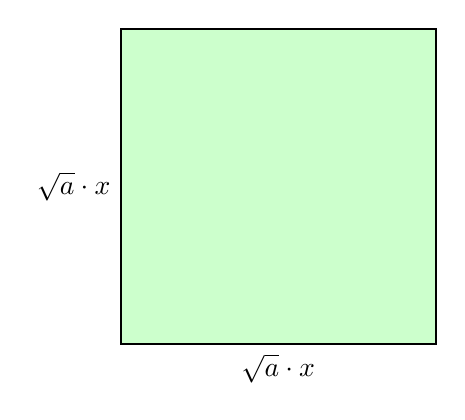
\begin{tikzpicture}[thick, scale=1]
        \fill [color=green,opacity=0.2] (0,0) rectangle +(4,4);
        \draw (0,0) rectangle +(4,4);
        \path (0,0) -- (4,0) node[midway,below] {$\sqrt{a}\cdot x$};
        \path (0,0) -- (0,4) node[midway,left] {$\sqrt{a}\cdot x$};
    \end{tikzpicture}
\end{center}

那么我们应该如何表示 $bx$ 这一项呢?我们要把正方形扩展到更大的正方形;这就是配方的意义。因此,我们需要围绕正方形构建一些矩形,这将有助于我们实现这一目标。让我们将 $bx$ 项代表的面积分成两个矩形,每个矩形的面积为 $\frac{b}{2}x$。由于矩形必须有一条边的长度为 $\sqrt{a} \cdot x$,并且我们希望矩形面积为 $\frac{b}{2}x$,因此另一条边长必然为 $\frac{b}{2\sqrt{a}}$: 

\begin{center}
    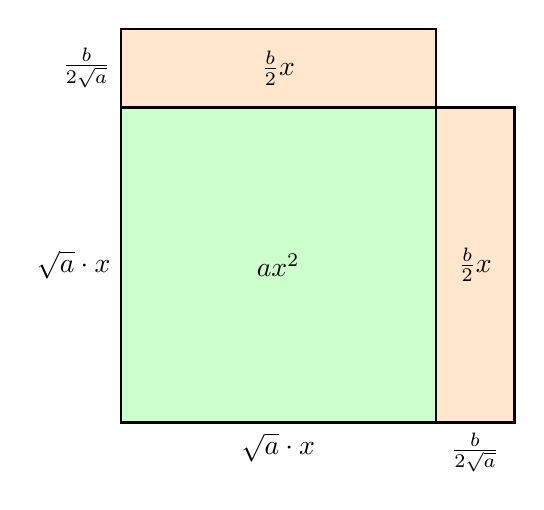
\begin{tikzpicture}[thick, scale=1]
        \fill [color=green,opacity=0.2] (0,0) rectangle +(4,4);
        \draw (0,0) rectangle +(4,4) node[pos=.5, align=center]{$ax^2$};
        \path (0,0) -- (4,0) node[midway,below] {$\sqrt{a}\cdot x$};
        \path (0,0) -- (0,4) node[midway,left] {$\sqrt{a}\cdot x$};

        \fill [color=orange,opacity=0.2] (4,0) rectangle +(1,4);
        \draw (4,0) rectangle +(1,4) node[pos=.5, align=center]{$\frac{b}{2}x$};
        \path (4,0) -- (5,0) node[midway,below] {$\frac{b}{2\sqrt{a}}$};

        \fill [color=orange,opacity=0.2] (0,4) rectangle +(4,1);
        \draw (0,4) rectangle +(4,1) node[pos=.5, align=center]{$\frac{b}{2}x$};
        \path (0,4) -- (0,5) node[midway,left] {$\frac{b}{2\sqrt{a}}$};
    \end{tikzpicture}
\end{center}

我们需要添加什么才能使上面的图形变成为一个正方形?我们发现只需在右上角填充一个小正方形即可。小正方形边长为 $\frac{b}{2\sqrt{a}}$,因此它的面积 --- 我们需要添加的项--- 为 $\frac{b^2}{4a}$。

\begin{center}
    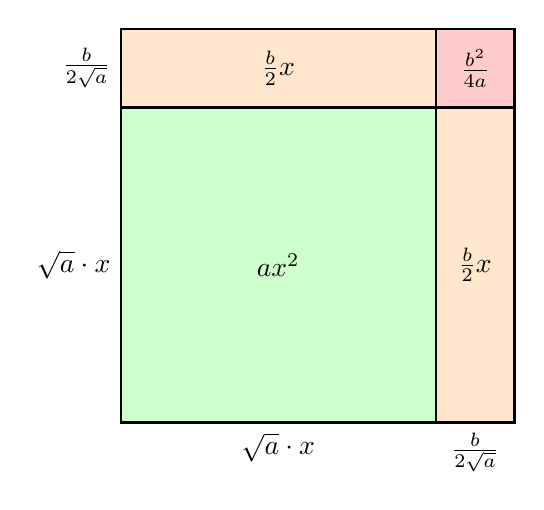
\begin{tikzpicture}[thick, scale=1]
        \fill [color=green,opacity=0.2] (0,0) rectangle +(4,4);
        \draw (0,0) rectangle +(4,4) node[pos=.5, align=center]{$ax^2$};
        \path (0,0) -- (4,0) node[midway,below] {$\sqrt{a}\cdot x$};
        \path (0,0) -- (0,4) node[midway,left] {$\sqrt{a}\cdot x$};

        \fill [color=orange,opacity=0.2] (4,0) rectangle +(1,4);
        \draw (4,0) rectangle +(1,4) node[pos=.5, align=center]{$\frac{b}{2}x$};
        \path (4,0) -- (5,0) node[midway,below] {$\frac{b}{2\sqrt{a}}$};

        \fill [color=orange,opacity=0.2] (0,4) rectangle +(4,1);
        \draw (0,4) rectangle +(4,1) node[pos=.5, align=center]{$\frac{b}{2}x$};
        \path (0,4) -- (0,5) node[midway,left] {$\frac{b}{2\sqrt{a}}$};

        \fill [color=red,opacity=0.2] (4,4) rectangle +(1,1);
        \draw (4,4) rectangle +(1,1) node[pos=.5, align=center]{$\frac{b^2}{4a}$};
    \end{tikzpicture}
\end{center}

看呐!这与我们上面通过代数推导得出的项完全相同。通过添加它,我们可以将这些项分解为完全平方。只需要再将其也减去,以确保原表达式不变。

这是一个需要记住的有用技巧。它可以提醒你配方的过程动机以及如何实现它。不过,你应该思考一件事:为什么这种可视化表示有效?我们必须假设 $a, b > 0$ 才能画出这些图,那么为什么无论 $a$ 和 $b$ 是什么,通向公式都有效呢?

\subsubsection*{二次函数求根公式}

让我们回到求多项式的根的问题。具体来说,让我们回忆一下\textbf{二次函数求根公式}。你可能已经记住这个公式是``求解二次方程''的一种方法,但你知道它为什么有效吗?让我们试着弄清楚吧!一般来说,我们从以下形式的二次多项式开始
\[p(x) = ax^2 + bx + c\]
其中 $a \ne 0$(否则,它就不是二次多项式),并且我们想要求 $p(x) = 0$ 时 $x$ 的值。(你是否尝试过回答我们上面提出的关于此类多项式有几个根的问题?在以下推导过程中请记住这些概念。)将该多项式因式分解为线性因子很麻烦,所以我们使用上面介绍的方法:配方。该方法的好处是,我们可以设置 $p(x)=0$,并在配方后重新整理项来求解 $x$。观察:
\[0 = p(x) = ax^2 + bx + c =a\Big(x+\frac{b}{2a}\Big)^2+\Big(c- \frac{b^2}{4a}\Big)\]
化简可得
\[\frac{b^2}{4a} -c = a\Big(x+\frac{b}{2a}\Big)^2\]

现在,我们要开始``撤消''此处的配方来求解 $x$,这需要对两边求平方根。但如果 $\frac{b^2}{4a} -c < 0$ 呢?我们根本无法求平方根!如果 $\frac{b^2}{4a} -c = 0$ 呢?会有问题吗?当 $\frac{b^2}{4a} -c > 0$ 时会有什么问题吗?这些问题与我们之前关于多项式可能有的根数相关。你可能已经(正确地)推断出二次多项式最多可以有两个根,但在这里我们发现二次多项式可能有一个或零个根(及其原因)!

\begin{itemize}
    \item 当 $\frac{b^2}{4a} -c < 0$ 时,那么 $x$ 的任何值都\emph{不}可能满足上面推导中的最后一行公式。因此,$p(x)$ 无实数根。
    \item 当 $\frac{b^2}{4a} -c = 0$ 时,那么对上面最后一行公式两边取平方根是完全有效的,但只会产生\emph{唯一一个 }$x$ 值:
    \begin{align*}
        \frac{b^2}{4a} -c = 0 &= a\Big(x+\frac{b}{2a}\Big)^2 \\
        0 &= x+\frac{b}{2a} \\
        x &= -\frac{b}{2a}
    \end{align*}
    \item 当 $\frac{b^2}{4a} -c > 0$ 时,此时,我们预期 $p(x)$ 有\emph{两个}根,因为两边取平方根会引入两个可能的解。一般来说,当我们遇到像 $s^2 = t$ 这种情况时,我们可以说唯一可能的解是 $s =\sqrt{t}$ 和 $s = -\sqrt{t}$,但我们必须同时考虑两者(通常将其写做 $s = \pm\sqrt{t}$)。在这种情况下求解 $x$ 得
    \begin{align*}
        \frac{b^2}{4a} -c &= a\Big(x+\frac{b}{2a}\Big)^2 \\
        \pm\sqrt{\frac{b^2-4ac}{4a}} &= \sqrt{a}\Big(x+\frac{b}{2a}\Big) = \sqrt{a}x+\frac{b}{2\sqrt{a}} \\
        -\frac{b}{2\sqrt{a}}\pm\frac{\sqrt{b^2-4ac}}{\sqrt{4a}} &= \sqrt{a}x \\
        -\frac{b}{2a}\pm\frac{\sqrt{b^2-4ac}}{\sqrt{4a^2}} &= x
    \end{align*}
    现在,我们必须小心对待之前进行的平方根观察。一般来说,$\sqrt{4a^2} = \pm2a$,但我们知道分子上的平方根项已经有一个相关的 $\pm1$ 因子,因此分母上的因子不会改变这一点。因此,我们可以得出结论
    \[x = -\frac{b}{2a}\pm\frac{\sqrt{b^2-4ac}}{2a} = \frac{-b\pm\sqrt{b^2-4ac}}{2a}\]
    这就是二次函数求根公式!
\end{itemize}

请记住,推导的最后一种情况是在 $\frac{b^2}{4a} -c > 0$ 的假设下进行的。当 $\frac{b^2}{4a} -c = 0$ 时,该公式依然适用吗?在这种假设下,我们是否可以执行与上面相同的步骤?为什么可以或者为什么不可以?

\subsubsection*{问题}

\begin{problem}
    找出 $a$ 的所有可能值,使 $x-a$ 是 $x^2+2ax-3$ 的因子。
\end{problem}
\begin{problem}
    找出 $b$ 的所有可能值,使得 $x^3 + b$ 可以被 $x + b$ 整除,没有余数。
\end{problem}
\begin{problem}
    对于任意自然数 $n$,因子 $x^n - 1$。
\end{problem}
\begin{problem}
    确定如下公式定义的 $x$ 的值
    \[x = \sqrt{2+\sqrt{2+\sqrt{2+\sqrt{2+\dots}}}}\]
    \begin{hint}
        尝试用 $x$ 本身来表示无限嵌套的平方根。
    \end{hint}
\end{problem}
\begin{problem}
    用配方法证明正数 $n$ 及其倒数之和始终大于或等于 $2$,并且唯一使和等于 $2$ 的数字是 $n = 1$。
    \begin{hint}
        求和,加减 $2$,然后重新整理。
    \end{hint}
\end{problem}
\begin{problem}
    如何求 $ax^4 + bx^2 + c$ 形式的四次多项式的根?
\end{problem}